\section{Problem Statement}
\label{sec:problem}

During our exploration of the different ways a connection between smart home and connected cars would make sense, we discovered that there are multiple areas for this:

\begin{figure}[ht]
	\centering
	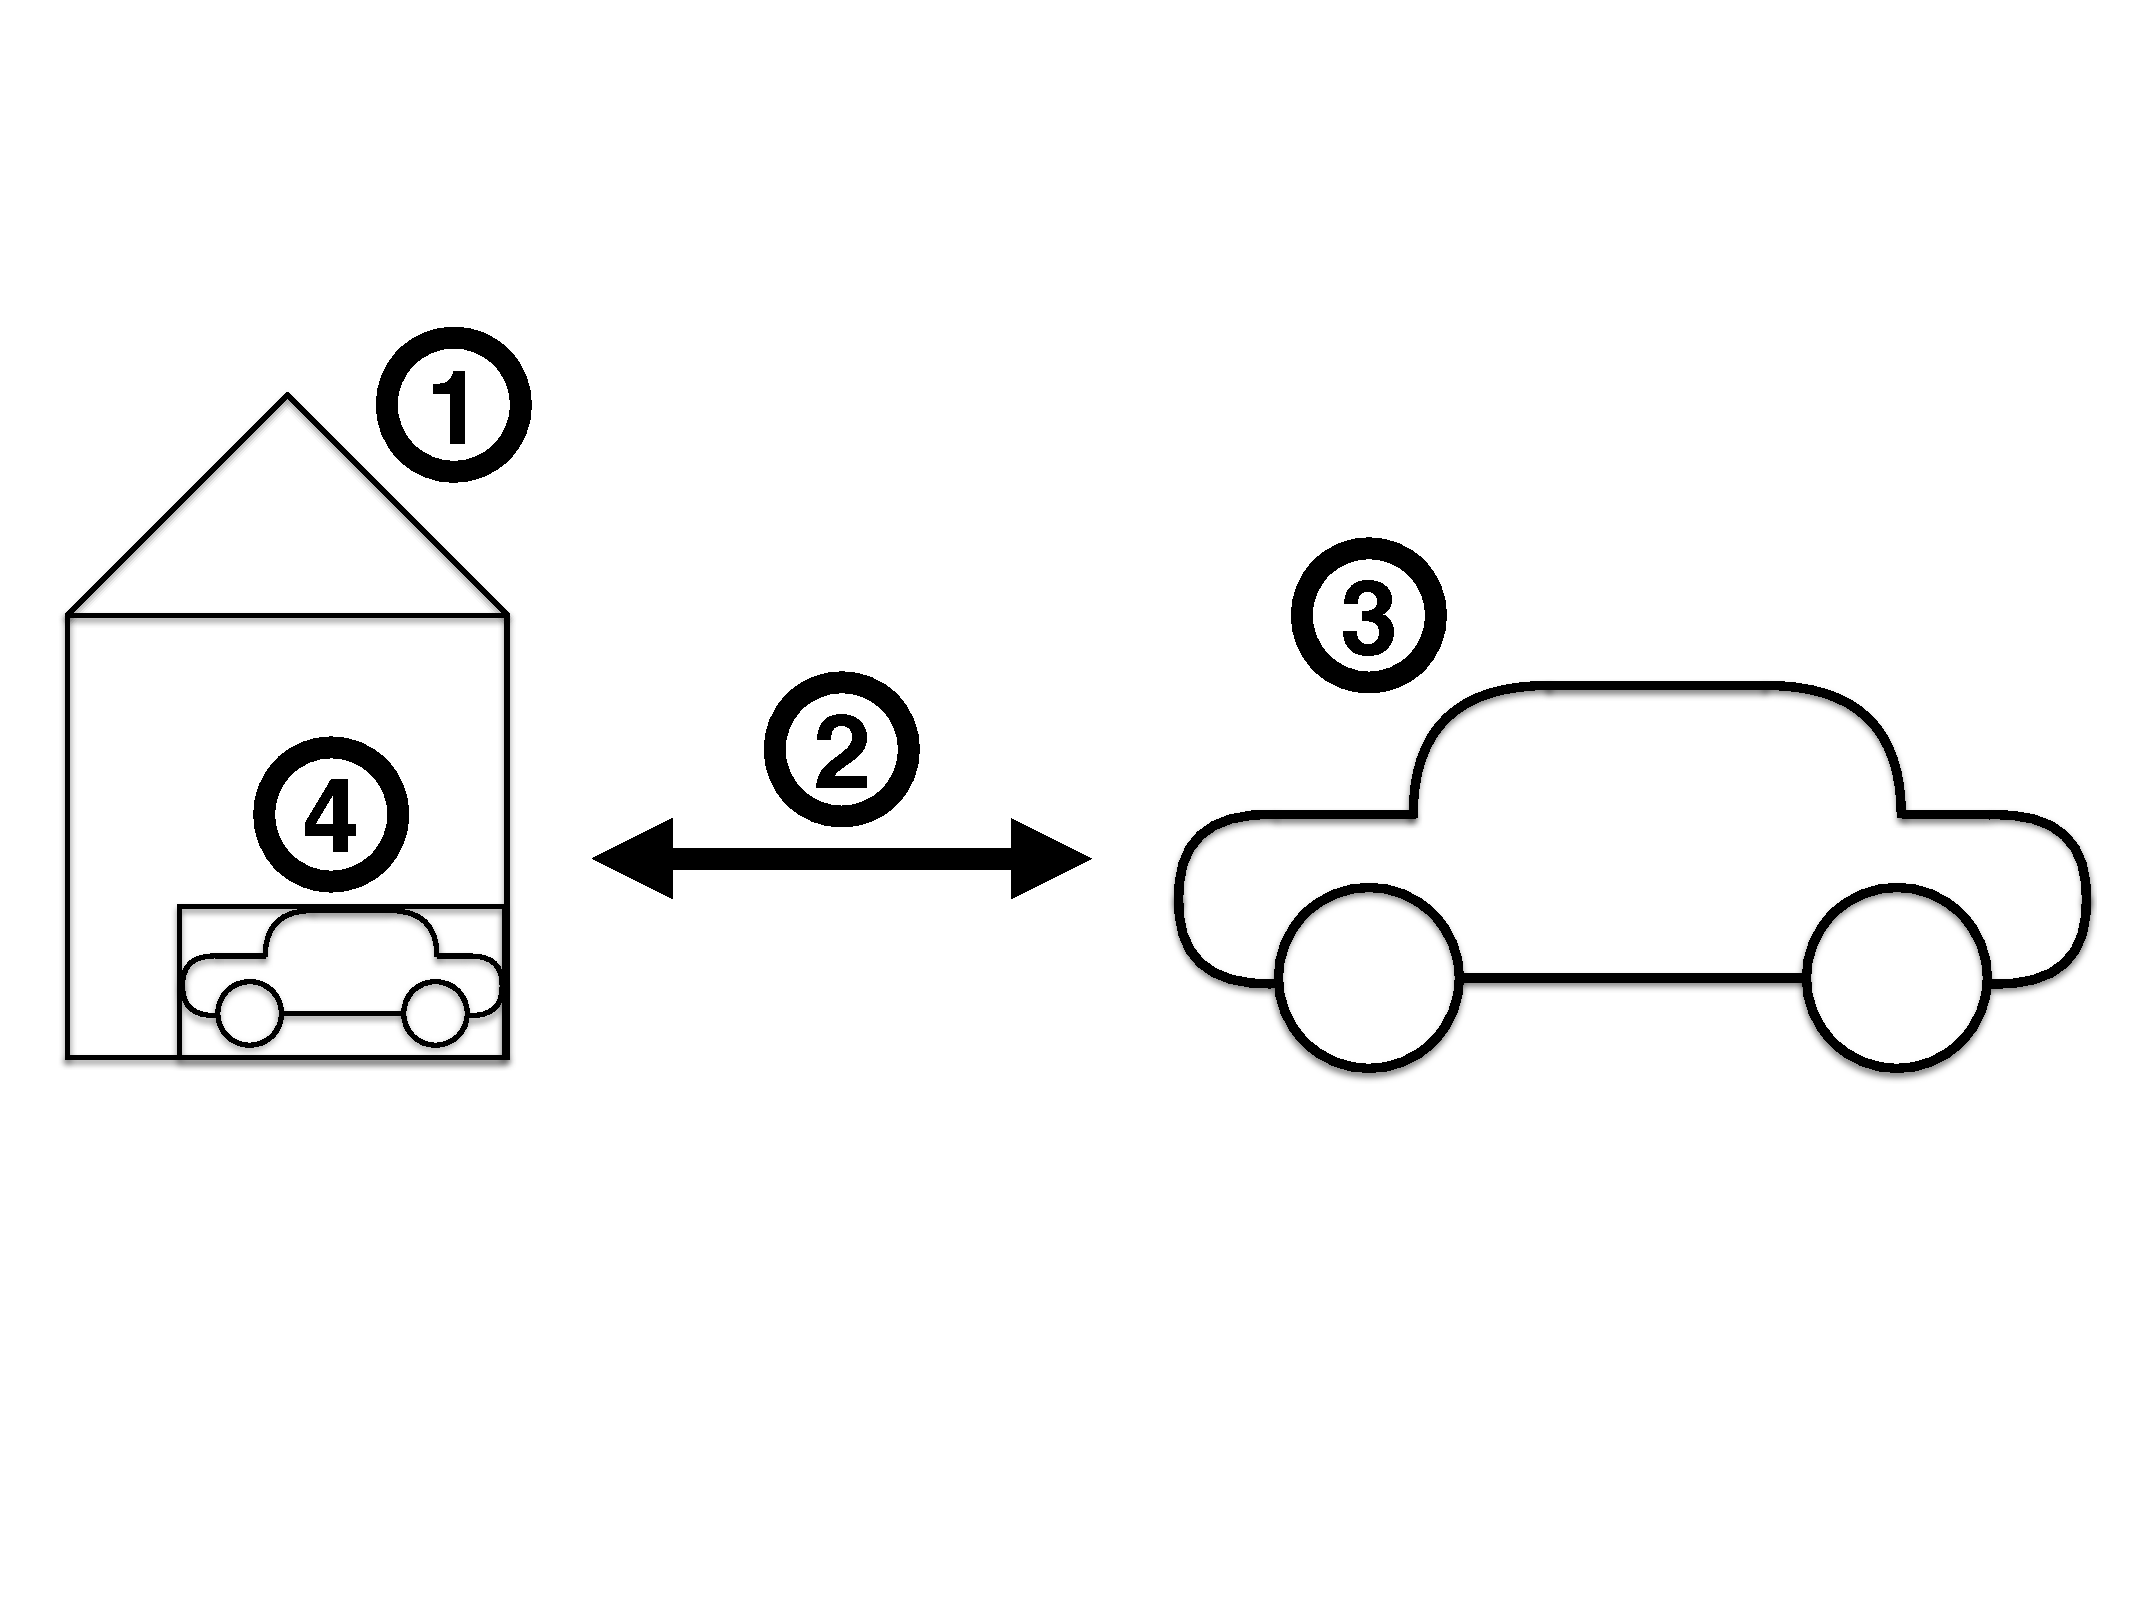
\includegraphics[width=\textwidth]{Figures/Development/CarAndHomeEquals}
	\caption{The four areas we identified for the combination of smart home and connected car}
	\label{fig:CarAndHome}
\end{figure}

\noindent
\\\textbf{1. Accessing the connected car from the smart home}
\\A subset of Audi owners take great pride in their ownership and therefore want to display that. They want the physical presence of the Audi brand to show their prestige, which also accounts for why most car manufacturers still design a heavy key fob even though technically it is not necessary to do so. When people leave their car, how could we still create an Audi ownership presence at home? It could be a physical product fixed at home, or a portable device that the user carries with them, or even some virtual products embedded in the user's cell phone or smart home system.

\noindent
\\\textbf{2. The transition between home and car}
% {Jonathan} This does not really make the case strong for the transition between home and car since entertainment is a mere luxury. Needs to be rewritten
%\\Car and home are two of the places where people spend most of their time (the third being their workplace), yet there are few connections between those two. People transit between car and home several times per day but the experience is not smooth enough. What if the home knew what the user was listening to on the radio before arriving home and turned on the home entertainment system when they walked in the door?


\noindent
\\\textbf{3. Accessing the smart home from the connected car}
\\There are a large number of people who spend hours in their cars everyday. For those, some technology that can improve their experience in traffic or on their long commute would be highly beneficial. Also, people sit and wait in their car to pick up their child from school or waiting for a client. In these cases, they want to be more productive, for example, reviewing documents for a meeting, checking emails, or messages. And as 
% Audi corrected us to not say autonomous and instead use "piloted"
piloted driving is around the corner, we can expect there would be more demands for in-car activity. Accessing the smart home from the connected car has some merits in these cases. Still, being productive inside a car is something that is less related to smart home in particular but is rather a concept that can be applied to many fields.

People who commute a lot in the car might also be interested in easier communication with families or friends. For example, letting the car tell the stay-at-home partner the expected time the other one would arrive home so that they can prepare dinner. Or the driver might be interested to take a look at what their kids are doing when he is in traffic to make sure they are not up to mischief.

\noindent
\\\textbf{4. The car as part or an extension of the smart home}
\\The car as part or an extension of the smart home is a truly futuristic concept that sees a physical integration between the two areas car and home. \todo{Dylan: This concept was tested in SU's darkhorse, and while interesting, did not seem like a viable approach. Is this something we really want to do? Or am I misinterpreting what is meant by physical integration of these spaces?\\
Jonathan: My understanding was that this part represents four viable areas that we could concentrate on but in the end we show that the transition between car and home is the best in our case}
\\\\
Based on our need finding and the factors mentioned above, we put our problem statement as: \textit{how might we improve the transition between home and car and make the Audi brand more present in the process?}.